\chapter{Design and Methodology}\label{chap:Methods }


% =============================================================================
\section{Visualization and User Interface}
% =============================================================================
Scholar Plot obtains the Impact Factor ($IF$) for a particular journal from our database. The data of Impact Factor is acquired from The Thomson Reuters Impact Factor - Web of Science. Based on all this information it constructs the plots as per the design outlined in the Visualization and User Interface section, using nvd3 library \cite{nvd3org}.


The NSF/NIH funding datasets are available at the respective US government websites in various file formats such as XML, CSV and so on \cite{nsf, nih}. We implemented a script to parse this massive XML dataset into our data structure that consists of AwardID, AwardAmount, First name, Last name, Investigator by RoleCode (Principal Investigator, Co-Principal Investigator and Former Principal Investigator), using XMLStarlet \cite{XMLStarlet}. We imported this data to our database using Toad DBMS tool. %We designed our relational database schema in MySQL.

\begin{figure}%[!htb]
\centering
  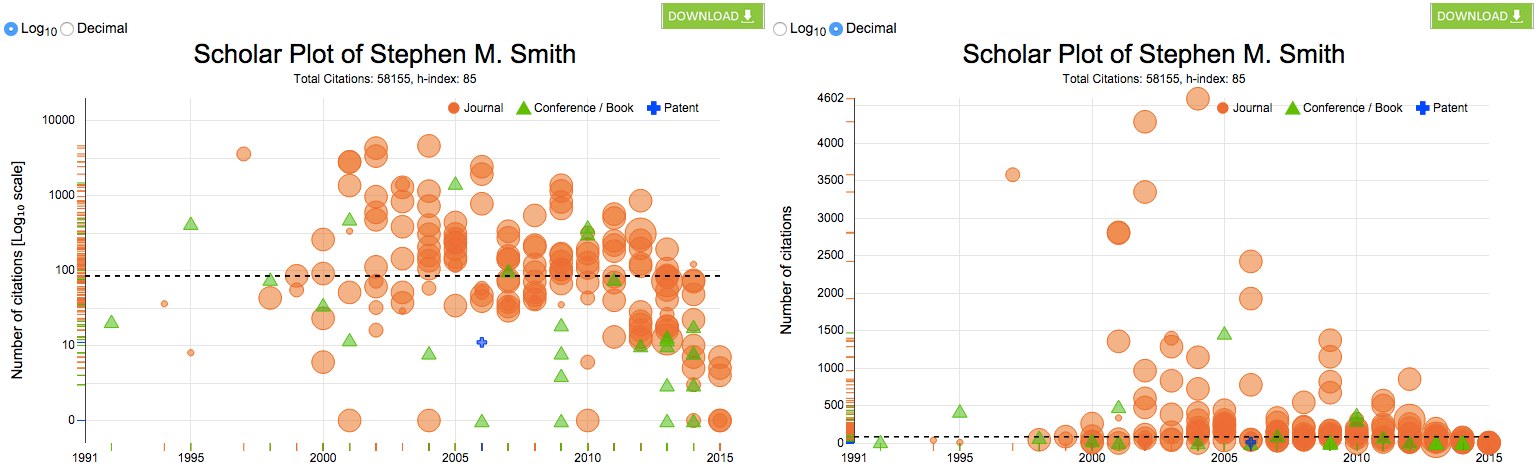
\includegraphics[width=1\columnwidth]{figures/fig_scaleView}
  \caption{The $log_{10}$ view and $decimal$ view: The radio button allows to switch between different scale views without reloading the entire page.}~\label{fig:fig-scale}
\end{figure}

\begin{figure*}
  \centering
  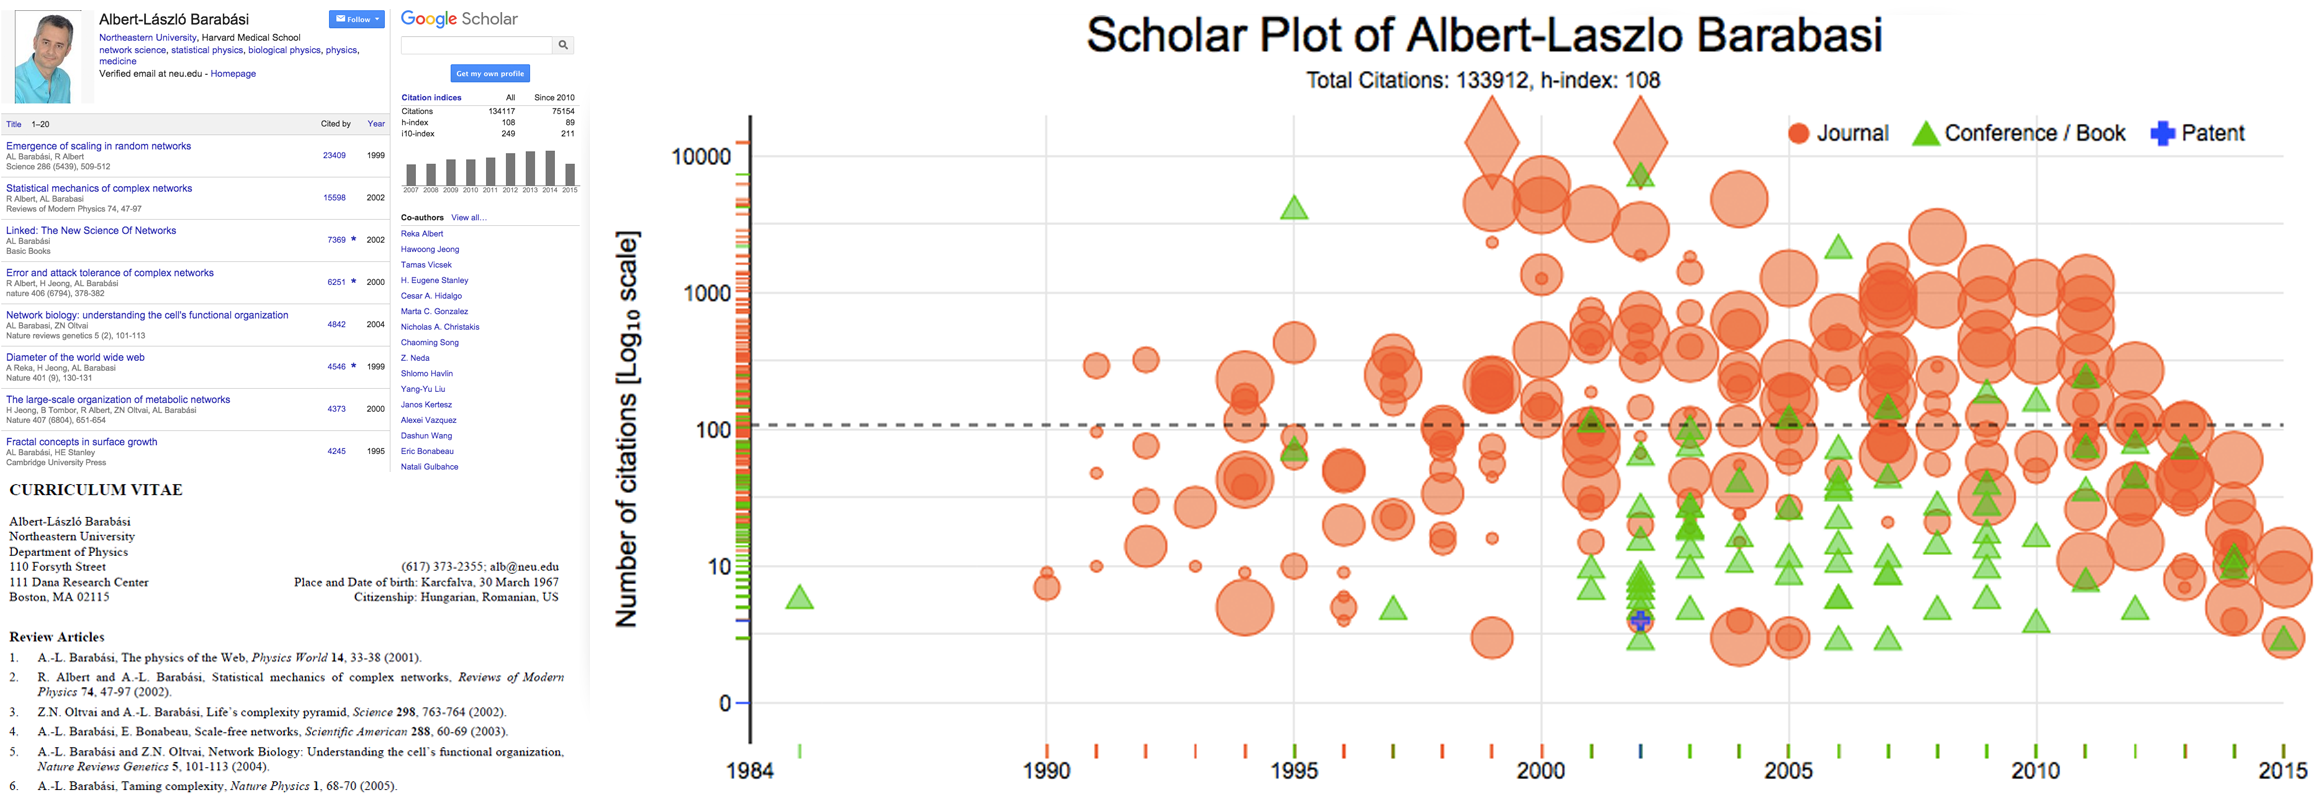
\includegraphics[width=2\columnwidth]{figures/fig_cv_google_scholarplot}
  \caption{An example of Scholar Plot - Visualizing Publication Data}~\label{fig:fig-publication}
 % \vspace{-1ex} 
\end{figure*}

Scholar Plot depicts the publications of an individual as a scatter plot and the NSF/NIH funding as a multiline plot. The publications are represented in a 2D diagram (number of citations vs. year of publication) with the {\it h}-index line (Figure \ref{fig:fig-publication}). The horizontal axis is time, starting with the year of the researcher's first publication ending with the current year. The vertical axis is the number of citations. The default plot is in $log_{10}$ scale. The user can also view the plot in the decimal scale by a toggle option using a radio button at the top left corner (Figure \ref{fig:fig-scale}). The log scale provides a standardized scale which helps to compare the plots of multiple scholars.



% --------------------------
\subsection{Visualizing Publication Data}
% --------------------------
Each publication $i$ is represented with a symbol. The center of the symbol has coordinates $(i_{PY}, i_{C})$, where $PY$ stands for Publication Year and $C$ for Number of citations obtained by the publication till date. The journals are represented as circles (orange) with area analogous to the impact factor the journal. The conferences / books are represented as triangles (green) and the patents as crosses (blue). By clicking at a symbol you can obtain the publication title, the year, the number of citations, the venue where published and its impact factor (if it is a journal), as well as a breakdown in the authorship, complete with the level of collaboration between the co-authors and the selected scholar (Figure \ref{fig:fig-tooltip}). The publication title also enables the user to navigate to the Google Scholar page for the selected paper. This helps to quickly verify and obtain further details of the selected publication. It makes user reach out to the PDF file directly if available. To enhance user experience, we customized the tooltip to give detailed information without overlapping the plots.

\begin{figure}[H]
\centering
  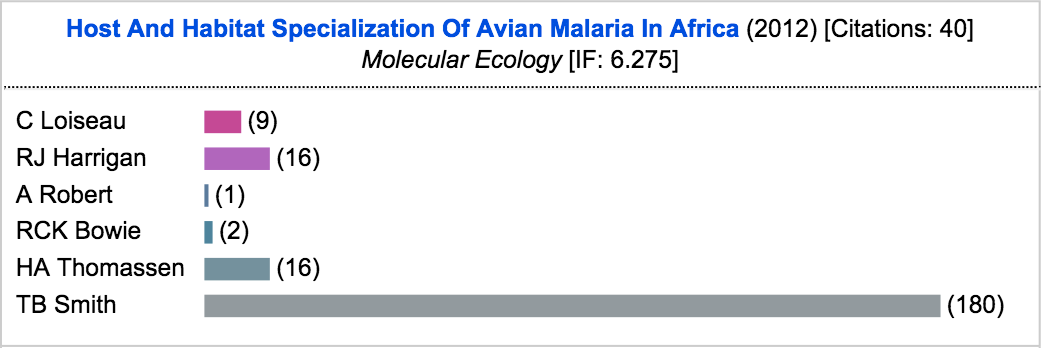
\includegraphics[width=1\columnwidth]{figures/fig_tooltip}
  \caption{An example of the tooltip: The publication title, the year, the number of citations, the venue where published, impact factor, the list of co-authors, the visual horizontal bars with the number of collaboration between the co-authors and the selected scholar.}~\label{fig:fig-tooltip}
 % \vspace{-1ex} 
\end{figure}

A dotted horizontal line on the plot denote the {\it h}-index of the scholar. We also denote those publications which earn greater than 10,000 citations with diamonds as they represent the great success in publications (Figure \ref{fig:fig-publication}). The title of the plot contains the name of the scholar and her/his total number of citations along with the {\it h}-index. At the top right corner of the plot, a legend shows the three different types of publications we distinctly display (Figure \ref{fig:fig-legend}).

\begin{figure}[!htb]
\centering
  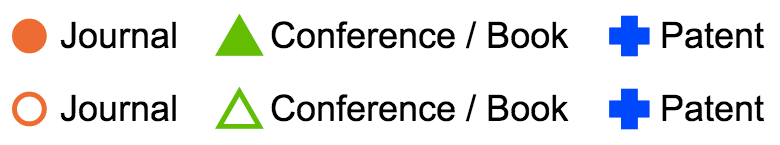
\includegraphics[width=0.9\columnwidth]{figures/fig_legend-toggle}
  \caption{The legend allows users to selectively view journals, conferences / books and patents.}~\label{fig:fig-legend}
 % \vspace{-1ex} 
\end{figure}

You can bring the journals, patents, and conferences / books in and out of the view by clicking at the respective legend. If there is an overlap between journals, conferences and patents, this feature can help the user to selectively view them. The user can also zoom into the plot for closer picture. Also note that the symbols are not completely opaque. So if there are multiple symbols which overlap, the user can see and interact with them by hovering the mouse over them appropriately.

% --------------------------
\subsection{Visualizing Funding Data}
% --------------------------
Scholar Plot also depicts the NSF/NIH funding of an individual as a multiline (Figure \ref{fig:funding}). Each breakpoint in the multiline corresponds to the individual's total amount in all NSF/NIH awards for the specific year. By pointing at a breakpoint you can obtain the NSF/NIH awards IDs, award amounts, and investigator's role. The total annual funding information per year is also available by clicking the legend. 

\begin{figure}[!htb]
  \centering
  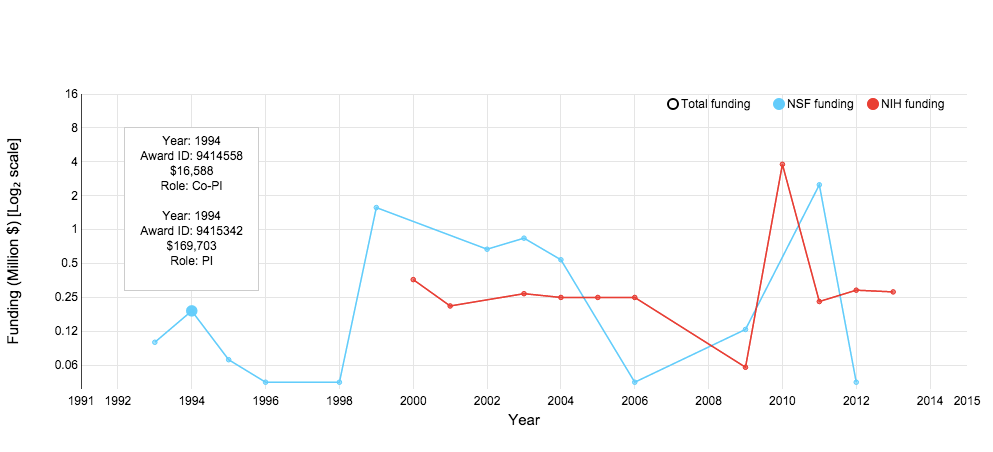
\includegraphics[width=1\columnwidth]{figures/fig_funding_default}
  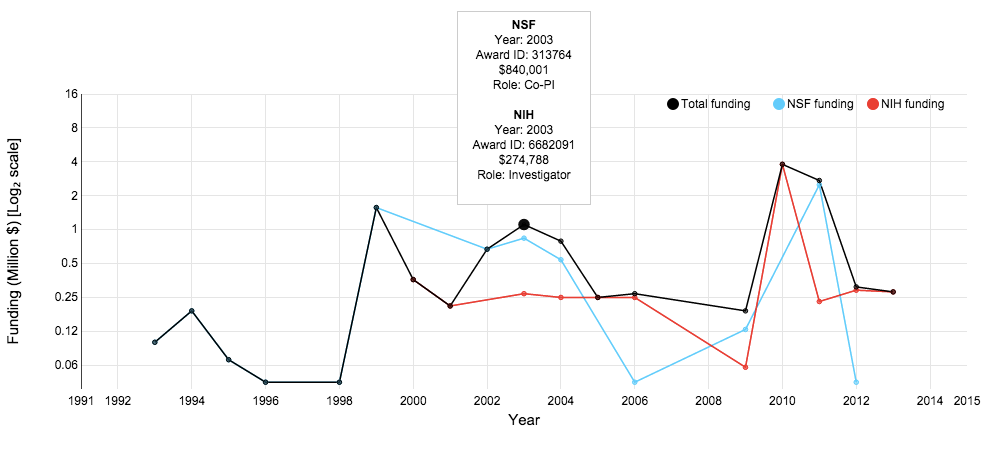
\includegraphics[width=1\columnwidth]{figures/fig_funding_total}
  \caption{An example of Scholar Plot - Visualizing Funding Data}~\label{fig:funding}
  % \vspace{-2ex} 
\end{figure}



%% --------------------------
%\subsection{Disk Size - How to determine the size of disks}
%% --------------------------
%We wanted to plot to visualize more efficiently with different size of disk for Journal publications that tells the different ranking of Journal by Impact Factor Index. To do this, we analyzed the data set of JCR 2013 IF and run quartile function as a useful concept in statistics to determine the size of disks in Scholar Plot. Based on this number, the system will decide the size of plot of each journal data and plot it in real-time. The quartile values are shown in table Table~\ref{tab:table1}. The maximum number from descriptive is 153.459 through. 
%
%\begin{table}
%  \centering
%  \begin{tabular}{c c}
%    \toprule
%    \multicolumn{2}{c}{\small{\textbf{ JCR Data (Impact Factor 2013) }}} \\
% 
%    {\small\textbf{Quartiles}}
%    & {\small \textit{IF}} \\
%    \midrule
%    Q1 & 0.67 \\
%    Q2 & 1.36 \\
%    Q3 & 2.47 \\
%    Q4 & 51.66 \\
%    \bottomrule
%  \end{tabular}
%  \caption{Table captions should be placed below the table. We
%    recommend table lines be 1 point, 25\% black. Minimize use of
%    unnecessary table lines.}~\label{tab:table1}
%\end{table}

%Scholar Plot gives a snapshot of the individuals profile in a concise manner.
To place the plots in your personal CV or on your web page we provide a download button at the top right corner of the plot (Figure \ref{fig:fig-scale}). This function enables the user to download plots in a zip file. It includes high resolution vector images in SVG (Scalable Vector Graphics) format of the publication and funding plots.

Scholar Plot also has a projection of the data on the y-axis depicted by small horizontal colored lines. For example, we can clearly see that journals contribute to the {\it h}-index of scholar in Figure \ref{fig:distribution} (a) and conferences / books contribute to the {\it h}-index of scholar in Figure \ref{fig:distribution} (b). We can clearly infer the scholar in Figure \ref{fig:distribution} (c)) has many patents. We can also infer the number of publications within a particular range of citations based on the density of the projected lines.

\begin{figure}[!htb]
\centering
\subfigure[]{%
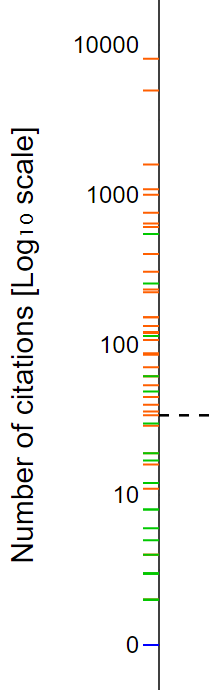
\includegraphics[width=0.23\columnwidth]{figures/fig_distribution_A}
}
\subfigure[]{%
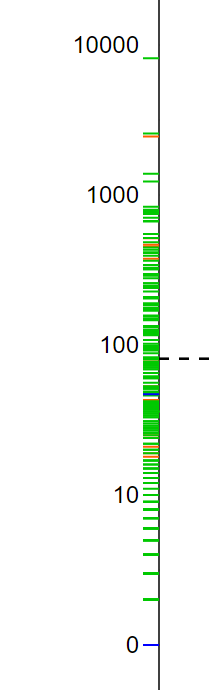
\includegraphics[width=0.23\columnwidth]{figures/fig_distribution_B}
}
\subfigure[]{%
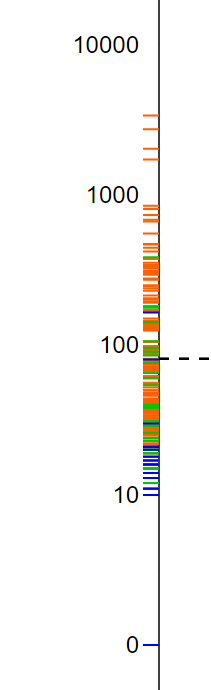
\includegraphics[width=0.23\columnwidth]{figures/fig_distribution_C}
}
\caption{Examples of y-axis projection for three different scholars.}~\label{fig:distribution}
  %\vspace{-1ex} 
\end{figure}

%\begin{figure}[!htb]
%  \centering
%  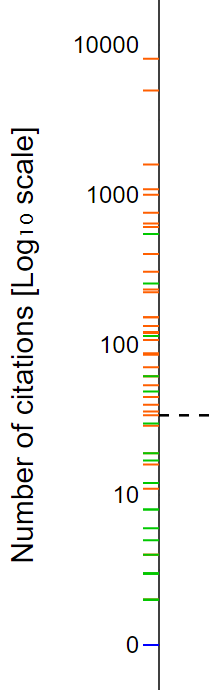
\includegraphics[width=0.2\columnwidth]{figures/fig_distribution_A}
%  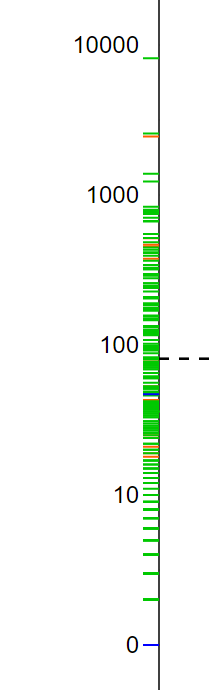
\includegraphics[width=0.2\columnwidth]{figures/fig_distribution_B}
%  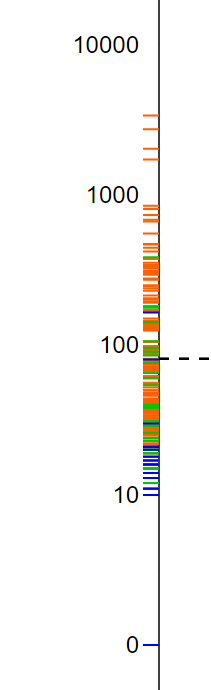
\includegraphics[width=0.2\columnwidth]{figures/fig_distribution_C}
%  \caption{Example with journals, conferences, and patents contributing to h-index}~\label{fig:distribution}
%\end{figure}

We improve user experience to enable users to quickly find and select from a pre-populated list of scholar names as they type. For each character the user enters, we display similar matching names on the dropdown list. Even entering the space (`` "), we display the 10 most recently inserted scholar's names. Scholar Plot follows the approach of responsive web design to provide optimal viewing based on the size of screen.


% =============================================================================
\section{System Architecture}
% =============================================================================
Scholar Plot is data visualization tool that uses HTML5, CSS3 and SVG to render a scholar's accomplishment at a glance. We created a MySQL database to store the mapping between the scholar names and their Google scholar IDs. We also designed and created database tables for NSF/NIH funding data. The user can search the name of the scholar in a text field. When the user starts to enter the name of the scholar, the names in our database which are similar to the entered name will be listed as a drop down list. We use jQuery and Ajax (asynchronous JavaScript and XML) method to have this feature, which connects to the database to get the list of names. If there are no matching/similar names, the user can also insert her/his Google Scholar ID to the database by one click event.

%Once the scholar's name selected, the user can run the application to see the visual results of the selected scholar's publications and fundings. Scholar Plot connects to the Web server to retrieve the necessary information.
The server-side application is implemented in PHP scripting language and MySQL. The HTTP protocol is used for communicating between client-side and server-side to get the basic information via JSON format (JavaScript Object Notation) and JSONP function (Figure \ref{fig:fig-arch}). Scholar Plot also uses htmlSQL library to parse Google scholar's page to extract user basic information \cite{htmlSQL}.
%, collecting for the publication title, the journal name, the co-authors' name, the year, and the citations. It also collects the {\it h-}index and the number of total citations from the top of the scholar's page up to 300 publications.

\begin{figure}
\centering
  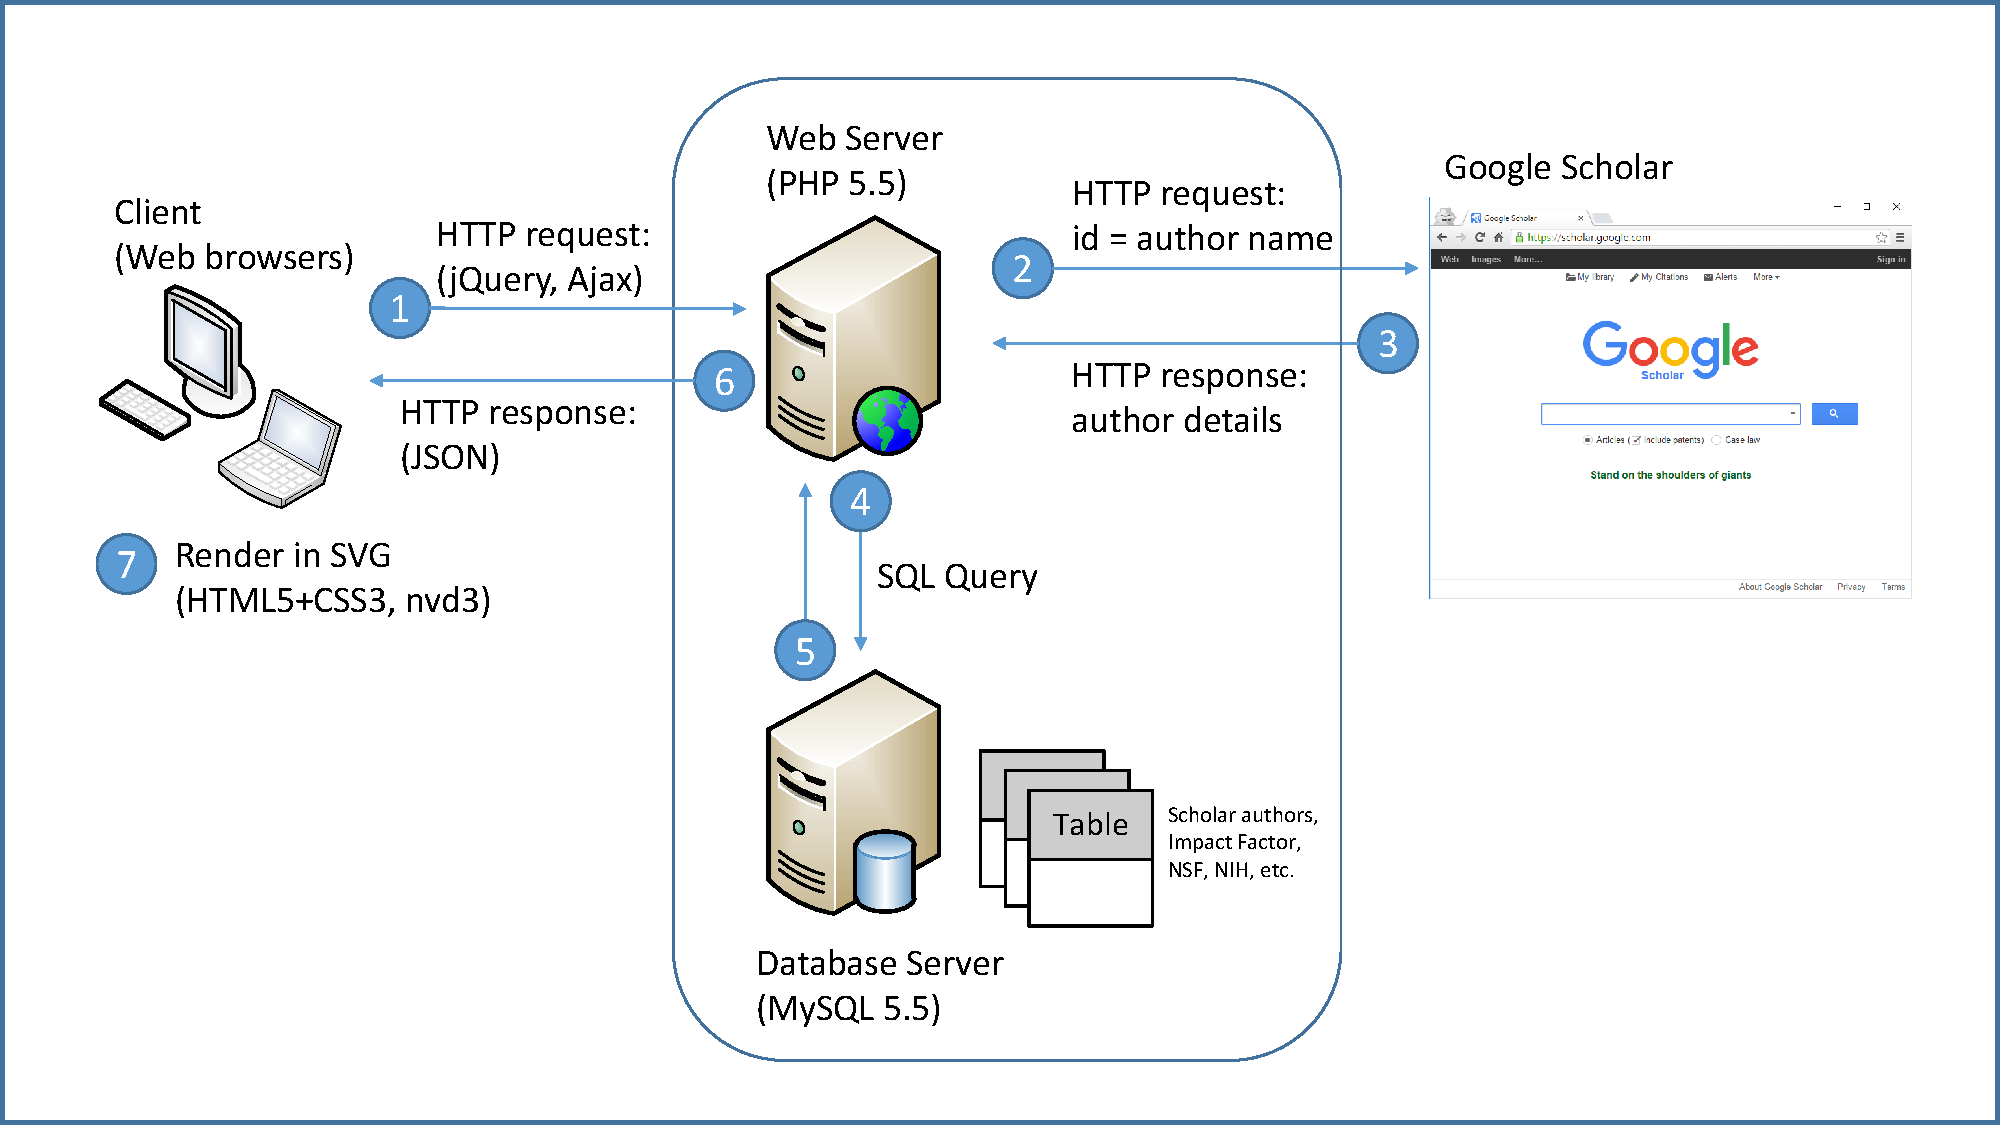
\includegraphics[width=1\columnwidth]{figures/fig_system_architecture.pdf}
  \caption{System Architecture of Scholar Plot.}~\label{fig:fig-arch}
%\vspace{-1ex} 
\end{figure}


% =============================================================================
\section{Name Disambiguation}
% =============================================================================
Google Scholar data has to be cleaned because it contains many non-english characters. We use regular expression to remove the invalid special characters and translate phonetic characters to english alphabets. We designed and implemented Algorithm \ref{alg:name} to match the author names in Google Scholar with those in NSF/NIH data. This process helps to improve the quality of results. 

\begin{algorithm}
\caption{Name disambiguation}\label{alg:name}
\begin{algorithmic}[1]
\Procedure{Searching for Author Name}{}
\State $\textit{FirstName} \gets \text{first name in Google Scholar }$
\State $\textit{LastName} \gets \text{last name in Google Scholar }$
\State $\textit{MiddleInitial} \gets \text{middle initial in Google Scholar }$
\If {$lastNameInFundingData = LastName$}
\If {$firstNameInFundingData = FirstName$} 
\If {$MiddleInitial$ is null } 
{\Return true}
\Else{
\text{Search for} ($MiddleInitial, FirstName$) and ($FirstName, MiddleInitial$) 
\If { $found$} \Return true
\Else{ \Return false}
\EndIf
}
\EndIf
\EndIf
\EndIf

\Return false
\EndProcedure
\end{algorithmic}
\end{algorithm}



% =============================================================================
\section{Name Disambiguation - Details}
\subsection{Within and across profile author name disambiguation}

Let $i$ be an index for the Google scholar profile researchers. Within each collaboration profile of $i$,  there are a set of $K_{0}$ raw name strings that you have extracted,  $Names_{k}$ indexed by $k_{i}$. We will use the fact that these strings are associated with profile $i$ in the process of name disambiguation across Google Scholar profiles. The following provides an outline of this procedure: \\


A) {\bf Clean last names:} 
Remove strings at end of all $Names_{k}$ that are not last names, and which may not consistently be listed for $k$, e.g. ``Jr.'', ``III'' etc. Hence, each name string  $Name_{k}$ consists ideally of a First name string $FN_{k}$, a Last name string $LN_{k}$, and possibly a Middle name string $MN_{k}$. \\

B)  {\bf Clean middle initial strings within each profile $i$:}  Within each $i$, search for inconsistencies in the use of $MN_{k}$. That is, possibly sometimes the author $k$ is listed as {\it Alexander M Petersen}, sometimes {\it Alexander Petersen}, and sometimes {\it Alexander Michael Petersen}. In this example the Last name string $LN_{k} = Petersen$ and the First name string $FN_{k} = Alexander$ are clearly consistent. But the Middle name string \{$\_$ , M, Michael\} causes some ambiguity if simple string comparison is used,  where $\_$ is a whitespace. 

%Hence, for each distinct  surname $FN_{k}$ and last name $LN_{k}$, map all $MN_{k}$ strings to the simplest representation $\hat X$ of just the middle name initials.\\

Then check to see how many different types of {\it Alexander} $\hat X$ {\it Petersen} occur within each $k$, where $\hat X$ is refers to the middle name. Use the following rules for when there are 2 or more types of $\hat W \hat X Petersen$.
 
 \begin{itemize}
 \item If there are only two  types of $Alexander \hat X Petersen$, with $\hat X=$ $\_$ or $M$, then map all of the $Alexander \hat X Petersen$ to $Alexander M Petersen$ for this $i$
 \item If there are only three types of $Alexander \hat X Petersen$, with $\hat X=$ starting with the same initial, $M\_$ or $M$, then map all of the $A\hat X Petersen$ to $Alexander Michael Petersen$ for this $i$
 \item If there are two or more types of $Alexander \hat X Petersen$, say $\hat X=O$ and $\hat X=P$, then keep these $X$ as they are.
 
%  \item However, if one of those types are a whitespace,  say $\hat X=O$ and $\hat X=P$  and $X= \_$, then we cannot know if the latter possibly corresponds to $O$ or $P$. This case shouldn't occur often. So we can use the simple heuristic that if there is any paper with $AO$ and $A$, then in this case the latter is actually $AP$, and so all $A\_$ are mapped to $AP$. If there are no papers that make obvious this distinction,  then compare the coauthors of $AO$ and $AP$  and $A \_$ within the profile of $i$. Map $A \_$ to $AP$ if they share more coauthors or map $A \_$ to $AP$ if they share more coauthors using the Jaccard Similarity measure to compare.
  
\end{itemize}

C)  {\bf Disambiguate coauthors $k$ across the Google Scholar profiles (connecting $i$):} Let  $k$ and $k'$ be coauthors in profiles $i$ and $i'$, respectively.   In this step we would like to identify $k$ and $k'$ that are likely the same person, $k=k'$, allowing us to connect the two profiles $i$ and $i'$ within the coauthor network.\\

 If $k$ and $k'$ have the same initials and same surname, then there is a possibility that they are the same individual. Also, if their full first name strings match, this is clearly very positive evidence of this. Let $A_{k,j}$ be the entire combination of First Name and Middle initial $FM_{k,j}$ with the surname $L_{k,j}$ (e.g. {\it Adam B Smith}, or {\it Adam \_ Johnson}) of the coauthor $j$ of the coauthor $k$. 

 \begin{itemize}
 \item If the full first name strings and the full last name strings are the same, $FN_{k,j}$=$FN_{k',j}$ and $LN_{k,j} = LN_{k',j}$ (e.g. Adam J. Johnson and Adam Johnson), and they both have at least one coauthors in common,  then they are considered the same coauthor. 
 \item If we don't have the added information of their full first names then we must rely more heavily on the information from their coauthors. If the first and last names are the same, $FM_{k,j}=FM_{k',j}$ and $LM_{k,j}=LM_{k',j}$, and there are more than 2 middle names with one of the middle name being empty, we do the following -
 
 We compute the number of coauthors in common of the empty middle name author with non-empty middle name authors by comparing the sets of coauthors, $\{j\}$.% and $\{j'\}$.
 
 We assign the empty middle name to that middle name for which there are more number of co-authors in common.
 
 \item If the first name of the author has a hyphen, we check for any other author having the same last name and the first name as the first word of the hyphenated word and middle name starting with the first letter of the second part of the hyphenated word. If any such pair of authors have at least one author in common, we update the first and middle name of the author with the hyphenated middle name to first name and middle name of the matched author.


\item If the first name of the author has only two letters, we check for any other author having the same last name and the first name starting with the first letter of the first name and middle name starting with the second letter of the first name. If any such pair of authors have at least one author in common, we update the first and middle names of the author with two letters to first and middle names of the matched author.
  
\end{itemize}
Google Scholar data has to be cleaned because it contains many non-english characters. We use regular expression to remove the invalid special characters and translate phonetic characters to english alphabets. We designed and implemented Algorithm \ref{alg:name} to match the author names in Google Scholar with those in NSF/NIH data. This process helps to improve the quality of results. 

